\section{PRINCIP VYPÍNACÍ OCHRANY ZAŘÍZENÍ TYPU LATCH při chybovém signálu}
Nastavení doby zpoždění, reset pomocí signálu UV

\begin{figure}[h]
   \begin{center}
     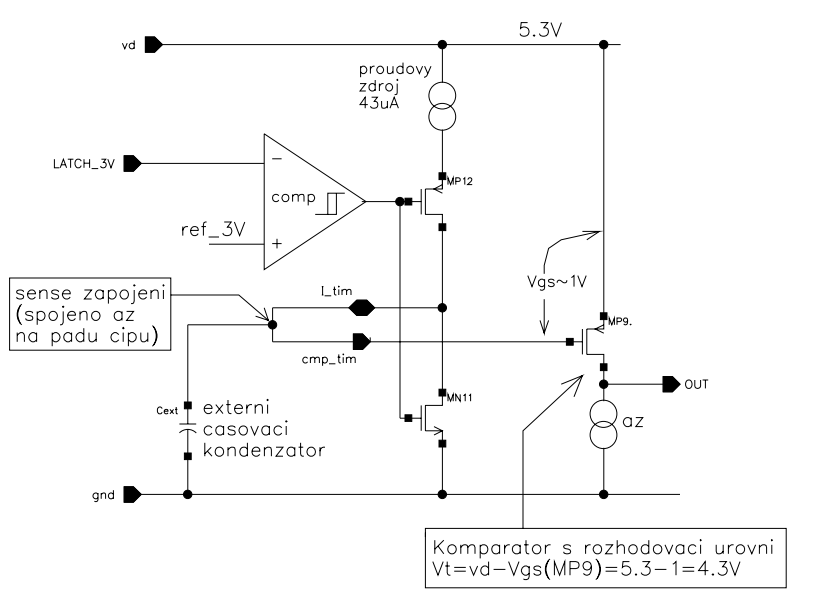
\includegraphics[scale=0.5]{images/Latch.png}
   \end{center}
   \caption{Principiální zapojení latch komparátoru s časovačem}
   \label{Latch}
\end{figure}

Pokud napětí na vstupu LATCH3V přesháne referenční úroveň 3 V, sepne comparátor comp(s hysterezí) proudový zdroj 43 $\mu$A. Tento proud začne nabíjet externí časovací kondenzátor Cext. Napětím na Cext je řízen jednoduchý komparátor, který je vytvořen z PMOS tranzistoru MP9 a aktivní zátěže OZ. Rozhodovací úroveň tohoto komparátoru je:
\begin{equation}
U_{t} = U_{d}-U_{gs}(MP9)
\end{equation}

Pokud napětí na C\textsubscript{ext} dosáhne hodnoty U\textsubscript{T}, změní se stav na výstupu OUT z úrovně H do úrovně L, stav L na výstupu OUT zablokuje celý sytém. K tomu je zapotřebí, aby chybový stav na výstupu LATCH3V (napětí vyšší, než 3 V) trval po dobu, za níž se C\textsubscript{ext} nabije na úroveň U\textsubscript{T} (z Obrázku \ref{Latch} je U\textsubscript{T} = 4,3 V). Tento čas je možné nastavit velikostí externího kondenzátoru C\textsubscript{ext}.

Pokud chybový stav zmizí dříve, než se C\textsubscript{ext} nabije na hodnotu U\textsubscript{T}, C\textsubscript{ext} je vybit pomocí NMOS MN11 a chybový stav na výstupu LATCH3V (napětí vyšší, než 3 V) se na výstupu OUT nijak neprojeví. Chybový stav je vlastně "filtrován" zpožděním - časem potřebným k nabití externího časovacího kondenzátoru na 4,3 V.

\begin{figure}[h]
   \begin{center}
     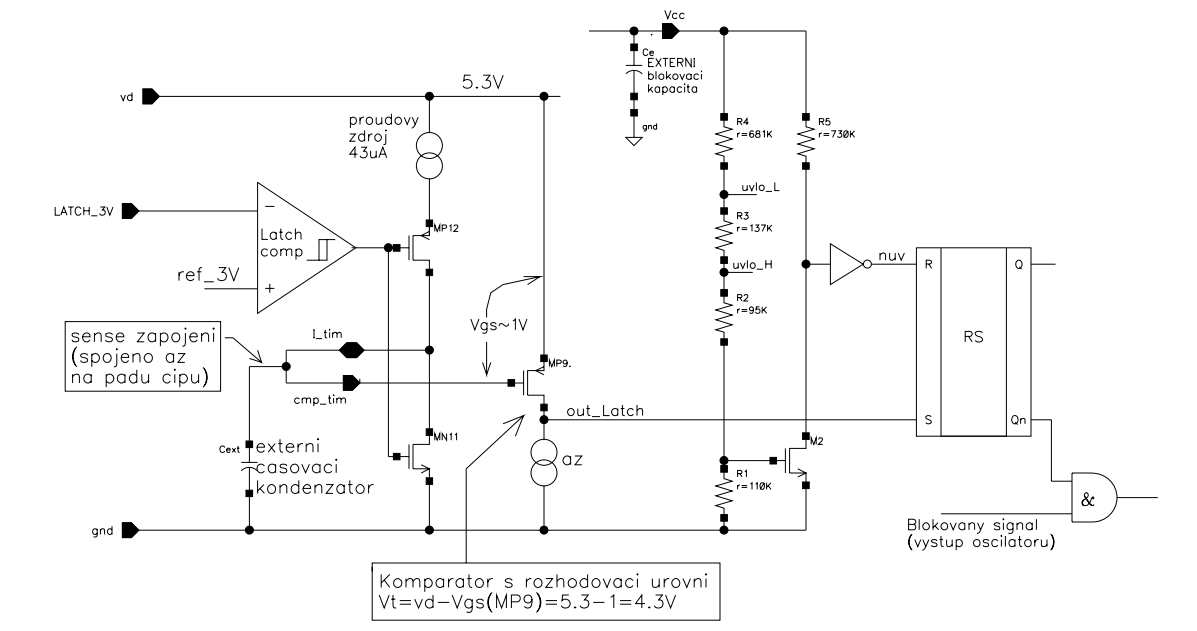
\includegraphics[scale=0.5]{images/Latch2.png}
   \end{center}
   \caption{Principiální zapojení obvodu "Chyba typu latch s časovačem"}
\end{figure}